%%%%%%%%%%%%%%%%%%%%%%%%%%%%%%%%%%%%%%%%%
% Beamer Presentation
% LaTeX Template
% Version 1.0 (10/11/12)
%
% This template has been downloaded from:
% http://www.LaTeXTemplates.com
%
% License:
% CC BY-NC-SA 3.0 (http://creativecommons.org/licenses/by-nc-sa/3.0/)
%
%%%%%%%%%%%%%%%%%%%%%%%%%%%%%%%%%%%%%%%%%

%----------------------------------------------------------------------------------------
%	PACKAGES AND THEMES
%----------------------------------------------------------------------------------------

\documentclass{beamer}

\mode<presentation> {

% The Beamer class comes with a number of default slide themes
% which change the colors and layouts of slides. Below this is a list
% of all the themes, uncomment each in turn to see what they look like.

%\usetheme{default}
%\usetheme{AnnArbor}
%\usetheme{Antibes}
%\usetheme{Bergen}
%\usetheme{Berkeley}
%\usetheme{Berlin}
%\usetheme{Boadilla}
%\usetheme{CambridgeUS}
%\usetheme{Copenhagen}
%\usetheme{Darmstadt}
%\usetheme{Dresden}
%\usetheme{Frankfurt}
%\usetheme{Goettingen}
%\usetheme{Hannover}
%\usetheme{Ilmenau}
%\usetheme{JuanLesPins}
%\usetheme{Luebeck}
\usetheme{Madrid}
%\usetheme{Malmoe}
%\usetheme{Marburg}
%\usetheme{Montpellier}
%\usetheme{PaloAlto}
%\usetheme{Pittsburgh}
%\usetheme{Rochester}
%\usetheme{Singapore}
%\usetheme{Szeged}
%\usetheme{Warsaw}

% As well as themes, the Beamer class has a number of color themes
% for any slide theme. Uncomment each of these in turn to see how it
% changes the colors of your current slide theme.

%\usecolortheme{albatross}
%\usecolortheme{beaver}
%\usecolortheme{beetle}
%\usecolortheme{crane}
%\usecolortheme{dolphin}
%\usecolortheme{dove}
%\usecolortheme{fly}
%\usecolortheme{lily}
%\usecolortheme{orchid}
%\usecolortheme{rose}
%\usecolortheme{seagull}
%\usecolortheme{seahorse}
%\usecolortheme{whale}
%\usecolortheme{wolverine}

%\setbeamertemplate{footline} % To remove the footer line in all slides uncomment this line
%\setbeamertemplate{footline}[page number] % To replace the footer line in all slides with a simple slide count uncomment this line

%\setbeamertemplate{navigation symbols}{} % To remove the navigation symbols from the bottom of all slides uncomment this line
}
\usepackage{listings}
\usepackage{graphicx} % Allows including images
\usepackage{booktabs} % Allows the use of \toprule, \midrule and \bottomrule in tables
\usepackage{xcolor}
\usepackage{balance}
\usepackage[utf8]{inputenc}  
\usepackage[T1]{fontenc}  
\usepackage{tikz}
\colorlet{punct}{red!60!black}
\definecolor{background}{HTML}{EEEEEE}
\definecolor{delim}{RGB}{20,105,176}
\colorlet{numb}{magenta!60!black}
\lstdefinelanguage{json}{
    basicstyle=\small\ttfamily,
    numbers=left,
    numberstyle=\scriptsize,
    stepnumber=1,
    numbersep=2pt,
    showstringspaces=false,
    breaklines=true,
    frame=lines,
    % backgroundcolor=\color{background},
    literate=
     *{0}{{{\color{numb}0}}}{1}
      {1}{{{\color{numb}1}}}{1}
      {2}{{{\color{numb}2}}}{1}
      {3}{{{\color{numb}3}}}{1}
      {4}{{{\color{numb}4}}}{1}
      {5}{{{\color{numb}5}}}{1}
      {6}{{{\color{numb}6}}}{1}
      {7}{{{\color{numb}7}}}{1}
      {8}{{{\color{numb}8}}}{1}
      {9}{{{\color{numb}9}}}{1}
      {:}{{{\color{punct}{:}}}}{1}
      {,}{{{\color{punct}{,}}}}{1}
      {\{}{{{\color{delim}{\{}}}}{1}
      {\}}{{{\color{delim}{\}}}}}{1}
      {[}{{{\color{delim}{[}}}}{1}
      {]}{{{\color{delim}{]}}}}{1},
}
\lstset{language=json}
%----------------------------------------------------------------------------------------
%	TITLE PAGE
%----------------------------------------------------------------------------------------

\title[Exploratory Testing]{Fostering the Diversity of Exploratory Testing} % The short title appears at the bottom of every slide, the full title is only on the title page

\author{Julien Leveau\inst{1}, Xavier Blanc\inst{2}, Laurent Reveillère\inst{2}, Jean-Rémy Falleri\inst{2}, Romain Rouvoy\inst{3}} % Your name

\institute[shortinst]{ CIS Valley\inst{1}, LaBRI\inst{2}, University of Lille\inst{3}} % Your institution as it will appear on the bottom of every slide, may be shorthand to save space

\date{\today} % Date, can be changed to a custom date

\begin{document}

\begin{frame}
\titlepage % Print the title page as the first slide
\end{frame}


%----------------------------------------------------------------------------------------
%	PRESENTATION SLIDES
%----------------------------------------------------------------------------------------

\begin{frame}
\frametitle{Exploratory Testing}
    
    \begin{columns}[T]

        \begin{column}{.35\textwidth}
            \itemsep 1.5em
            \textbf{Sessions} : \\
            \begin{itemize}
                \item Finding anomalies or usability issues.
                \item No scripted test cases.
                \item A group of human testers.
                \item A sub-part of the application.
                \item A fixed period of time.
            \end{itemize}
        \end{column}
        \begin{column}{.65\textwidth}
            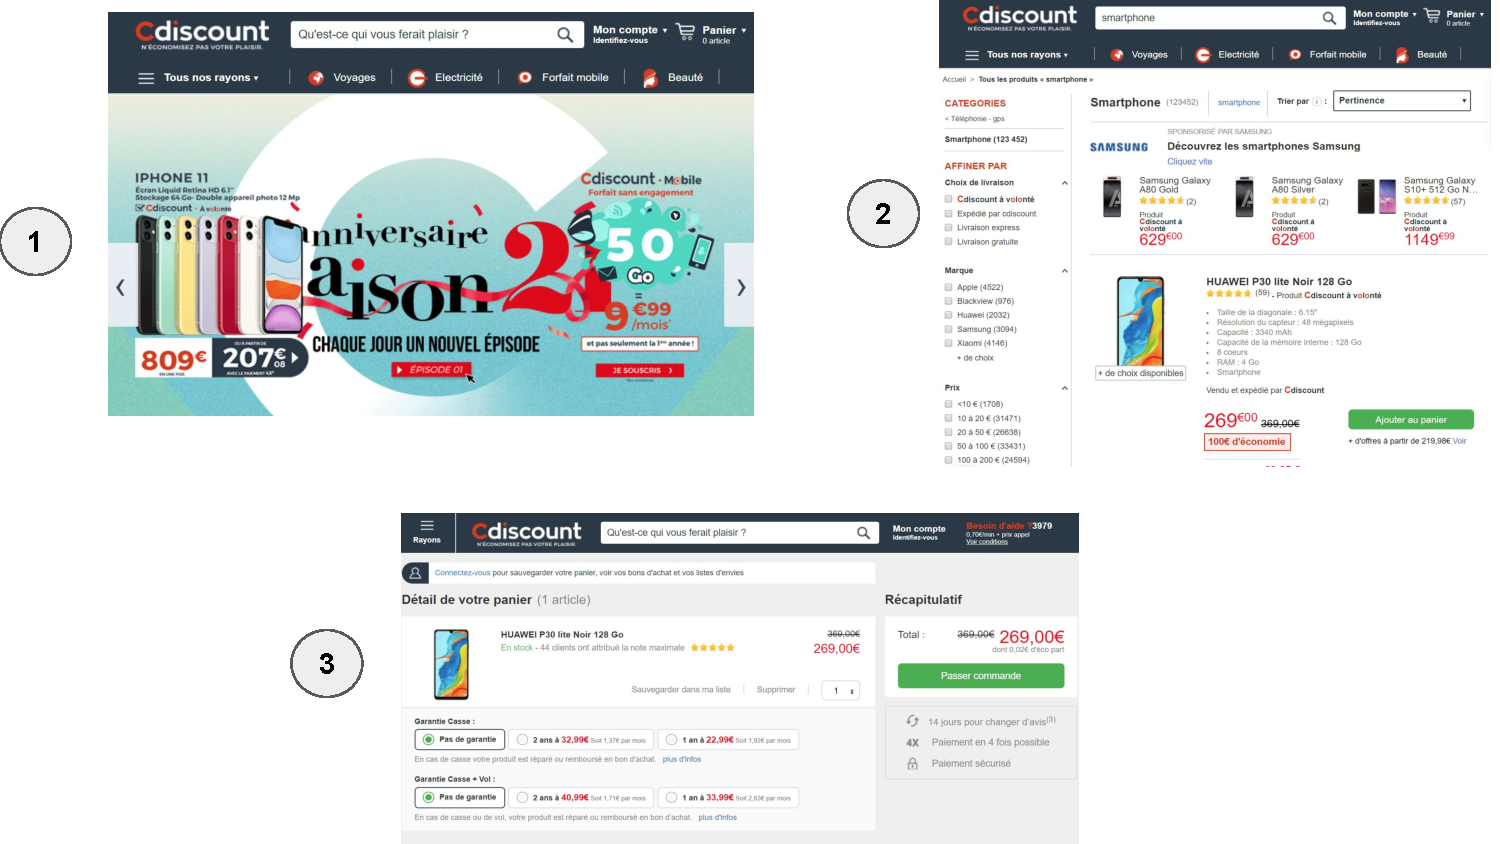
\includegraphics[width=\textwidth]{img/cdiscount.pdf}
        \end{column}
    \end{columns}
\end{frame}

%------------------------------------------------

\begin{frame}
    \frametitle{Problem}
    As a tester, how do I know if my exploration is helping to improve the coverage of the session ?
    \begin{itemize}
        \item Another tester may have already done this exploration.
        \item I may have forgotten to do an important test.
        \item I may have already done this test but I don't remember.
    \end{itemize}
    \end{frame}
    
    %------------------------------------------------

\begin{frame}
    \frametitle{Recording Explorations}

    \begin{columns}[T]
        \begin{column}{.35\textwidth}

        Identify the business actions : 
        \begin{itemize}
            \item Make research
            \item Add a product to the basket
            \item Open the basket
            \item Select the quantity
            \item Confirm the order
        \end{itemize}
        Define the granularity :
        \begin{itemize}
            \item Is the name of the product important ?
            \item Is the quantity value important ?
        \end{itemize}
        \end{column}
        \begin{column}{.65\textwidth}
            \vspace{10mm} %25mm vertical space
            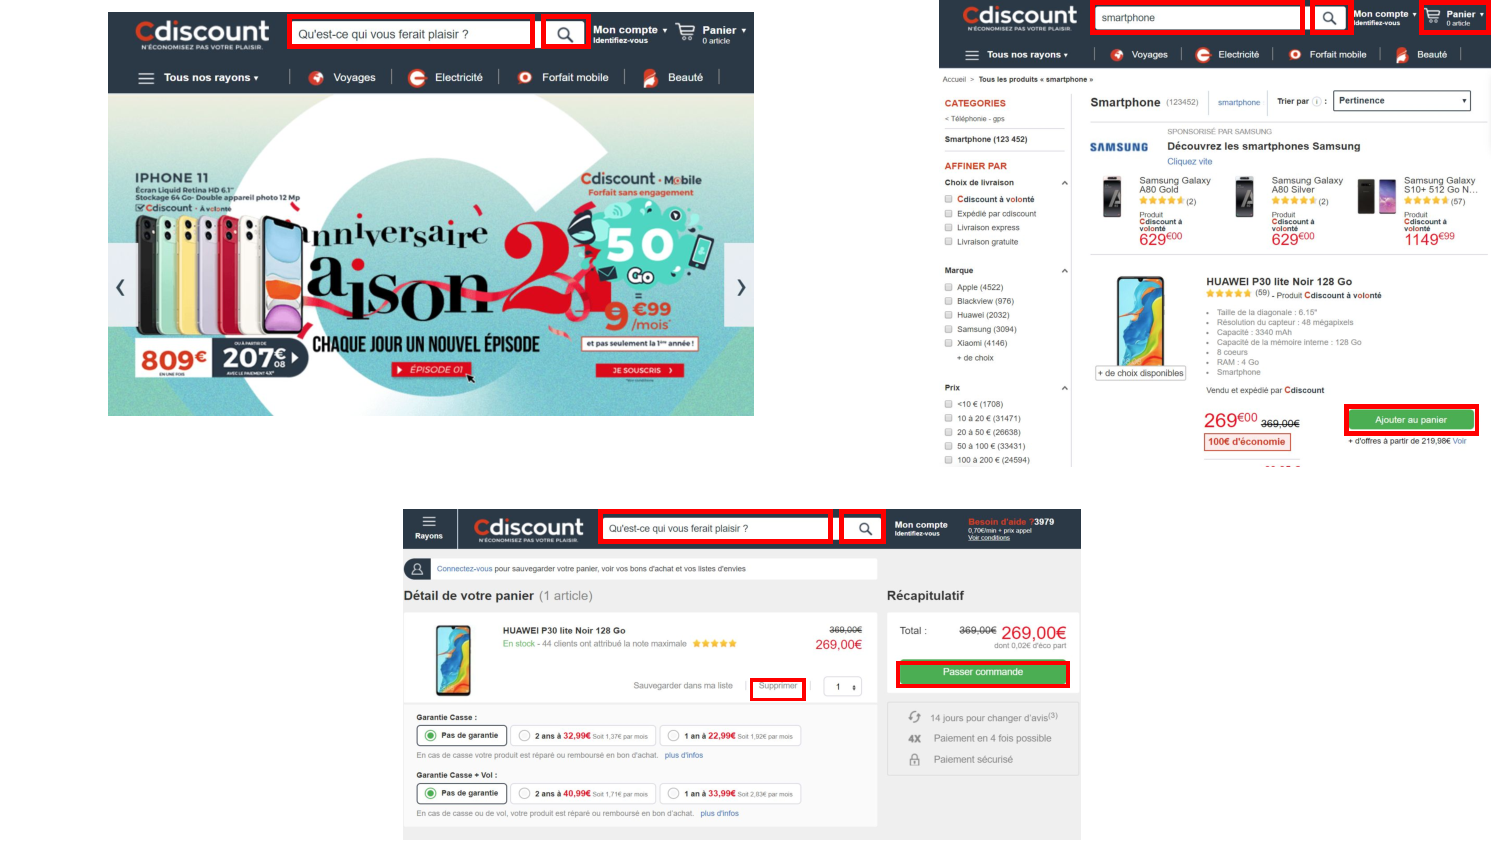
\includegraphics[width=\textwidth]{img/actions.pdf}
        \end{column}
    \end{columns}
\end{frame}
    

%------------------------------------------------



\begin{frame}
    \frametitle{Session}
    \textbf{Make the knowledge available to all the participants.} \\
    We record the actions made by the testers, and make a contextualized prediction for the next action. \\
    Warm color = High probability
    \vspace{1em}

    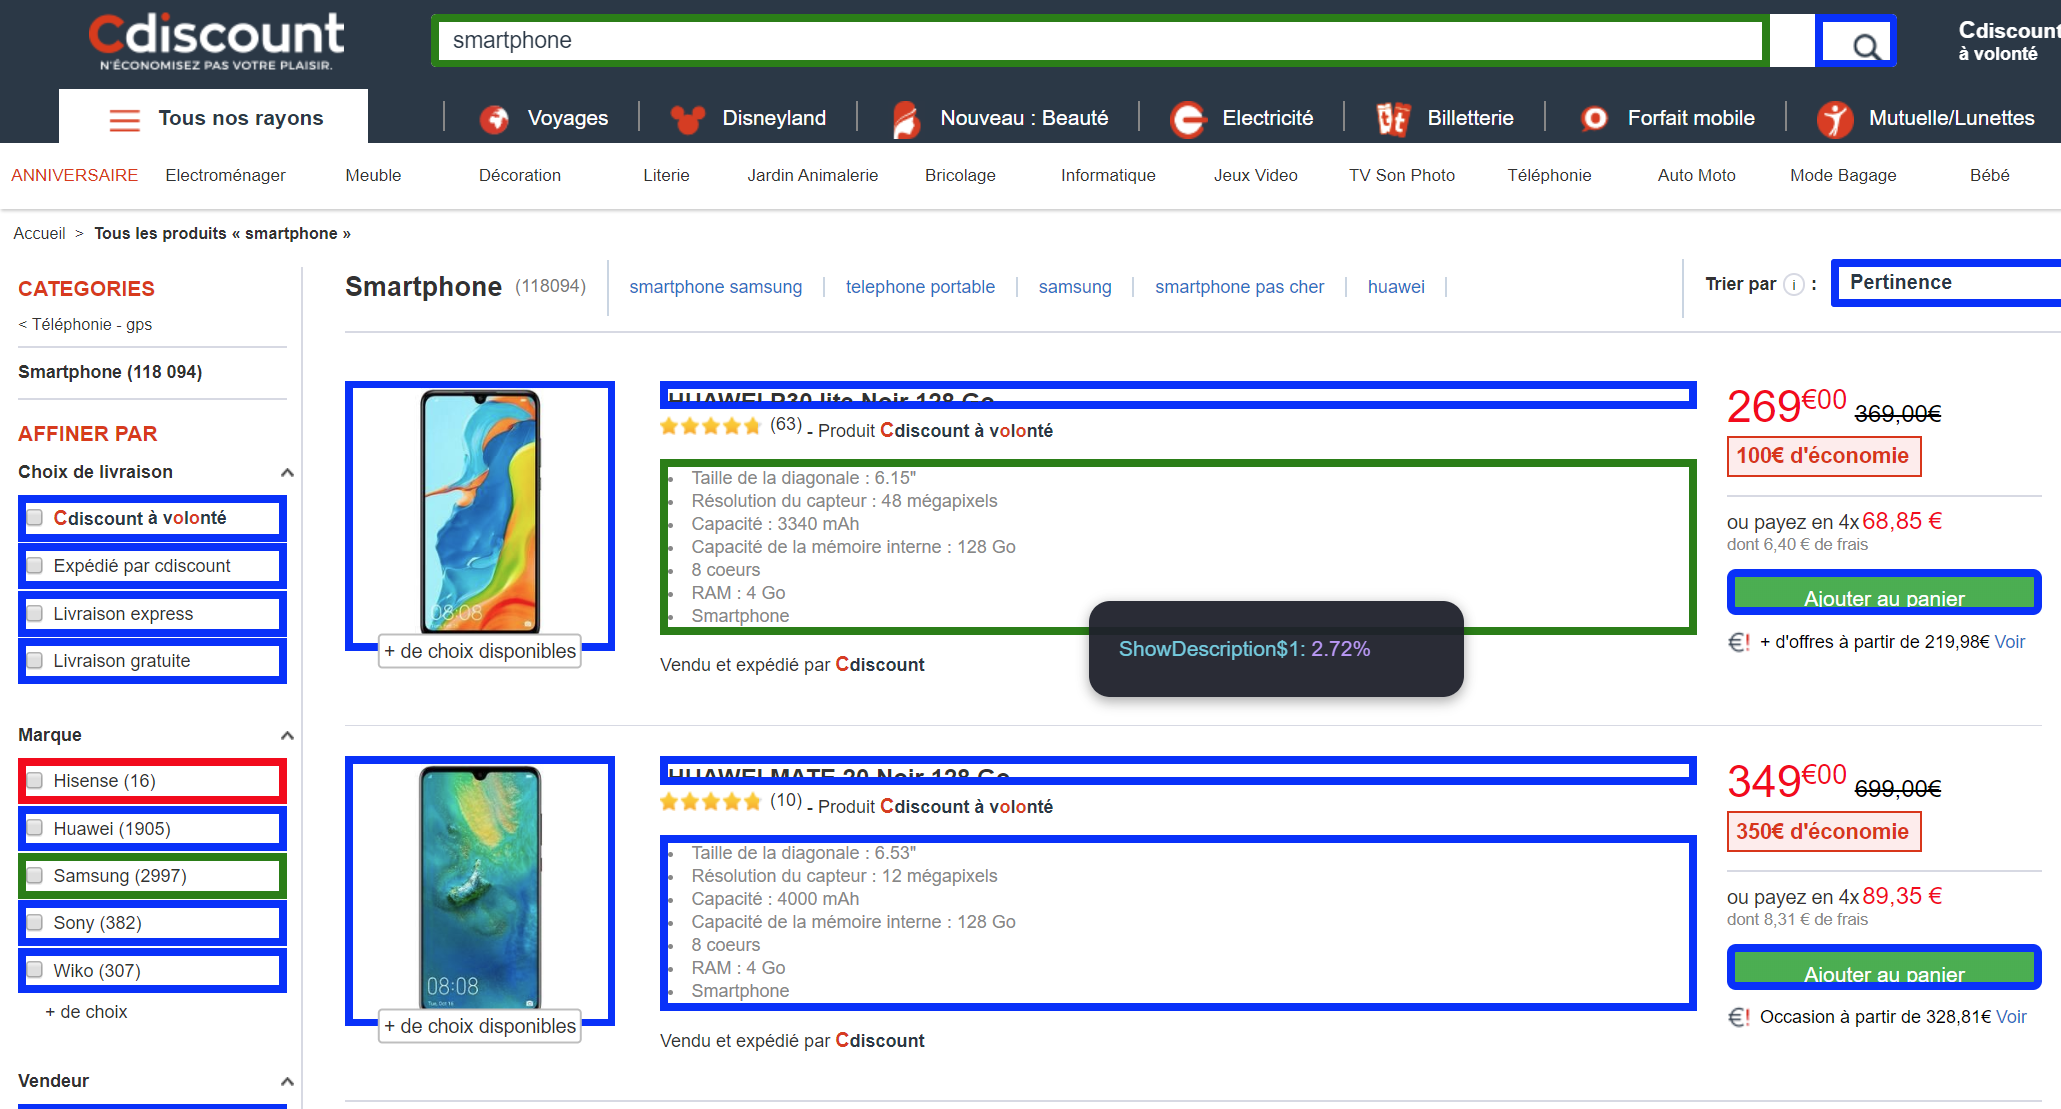
\includegraphics[width=0.7\textwidth]{img/plugin.png}
\end{frame}

\begin{frame}
    \frametitle{Prediction}
    Colors indicate the probability that the tester will make this action.  \\
    \begin{itemize}
        \item Click on blue : Add diversity.
        \item Click on red  : Follow the main path.
    \end{itemize}
    
    \textbf{Goal} : Assist the tester, pointing out how he or she can add diversity.
\end{frame}

\begin{frame}
    \frametitle{Validation}
    \textbf{Controlled Study}\\
    \begin{itemize}
        \item 39 participants in 13 groups.
        \item Ordering a product on cdiscount (30 actions).
        \item 10min assisted / 10min not assisted.
    \end{itemize}

    \textbf{Case Study}\\
    \begin{itemize}
        \item 8 testers from CIS Valley.
        \item An application estimated for a cost of 3000 man/days.
        \item A 15 min test session.
    \end{itemize}
\end{frame}

\begin{frame}
    \frametitle{Results}
    \begin{columns}[T]
        \begin{column}{.35\textwidth}
            Width : Number of different sequences. \\
            Depth : Average size of the traces. \\
            Diversity : $\frac{distinctNgrams}{totalOccurence}$ \\
        \end{column}
        \begin{column}{.65\textwidth}
            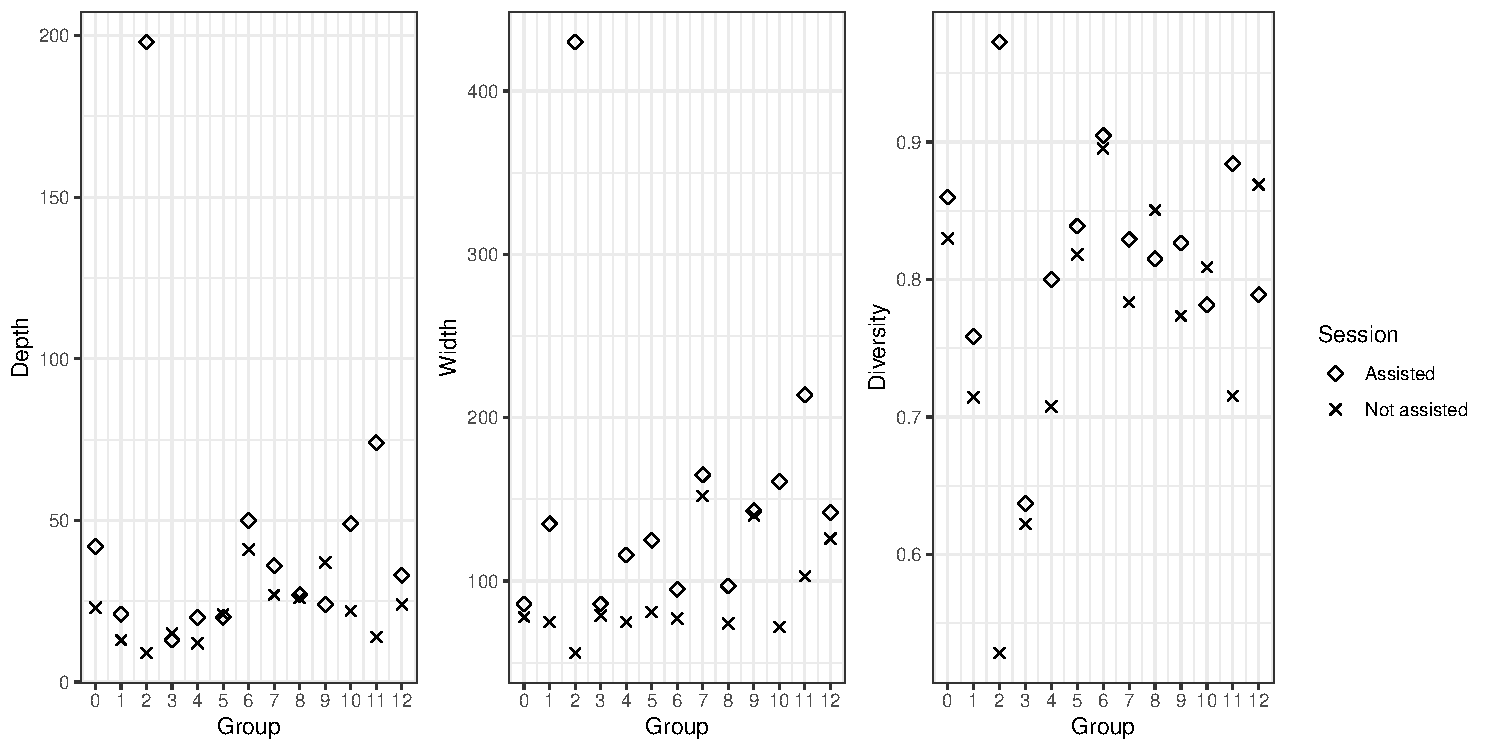
\includegraphics[width=1\textwidth]{img/controlled-study.pdf}
        \end{column}
    \end{columns}
\end{frame}


%------------------------------------------------

\end{document} 